
\documentclass[10pt]{article}
\usepackage[margin=2cm]{geometry}
\usepackage{booktabs}
\usepackage{longtable}
\usepackage{tabularx}
\usepackage{graphicx}
\usepackage{url}
\usepackage[T1]{fontenc}
\usepackage[utf8]{inputenc}
\Urlmuskip=0mu plus 1mu
\emergencystretch=3em

\title{Supplementary Information: Validation controlled imbalance aware learning for fine grained IoT intrusion detection}
\author{Junjie Zhang and Siyu Wang}
\date{}

\begin{document}
\raggedright
\maketitle

\section*{Supplementary Methods}

This supplementary file records overflow tables, result sources and reproduction commands for the Scientific Reports LaTeX submission package. Complete CSV files are supplied in the \path{supplementary_tables/} directory.

\section*{Supplementary Figure S1. CICIoT2023 SHAP feature contributions}

\begin{center}
\centering
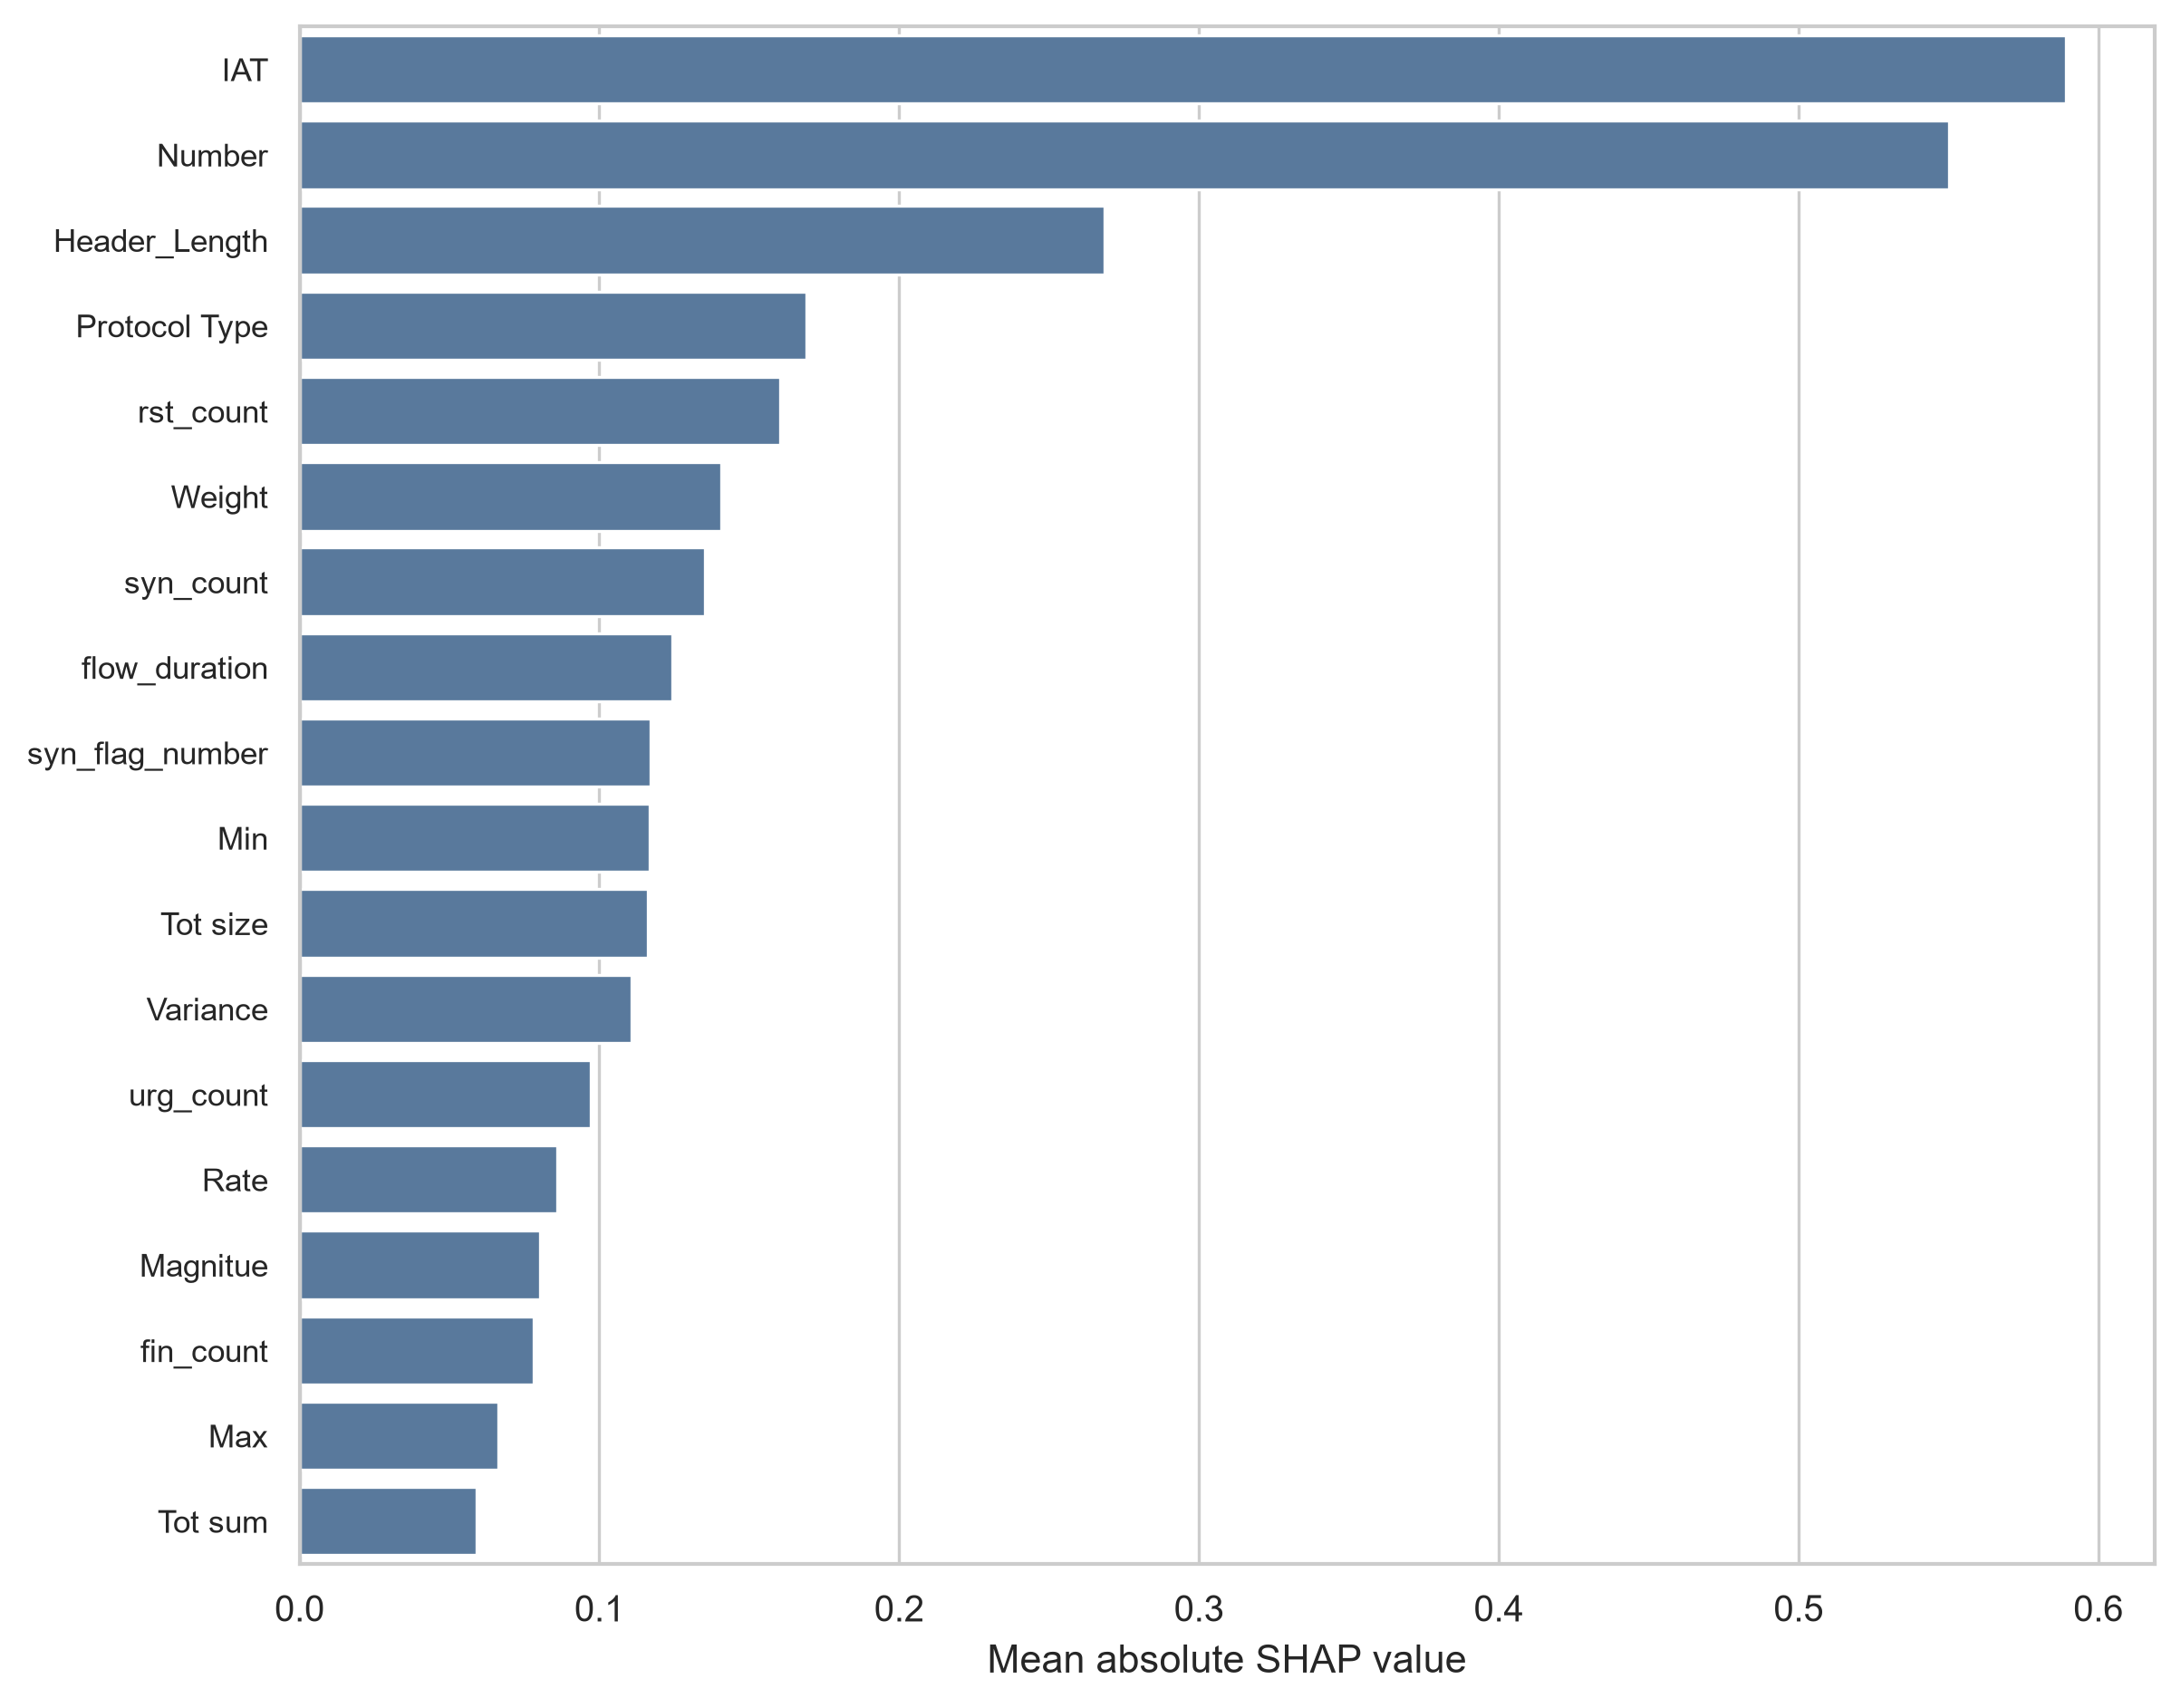
\includegraphics[width=0.82\linewidth]{figures/supplementary_figure_s1_ciciot_shap_top_features.png}
\par\smallskip
\small Mean absolute SHAP values for the highest-ranked features in the CICIoT2023 Borderline-SMOTE LightGBM component. The analysis is used for component-level attribution, not causal interpretation.
\end{center}

\section*{Supplementary Figure S2. CICIoT2023 alpha sensitivity}

\begin{center}
\centering
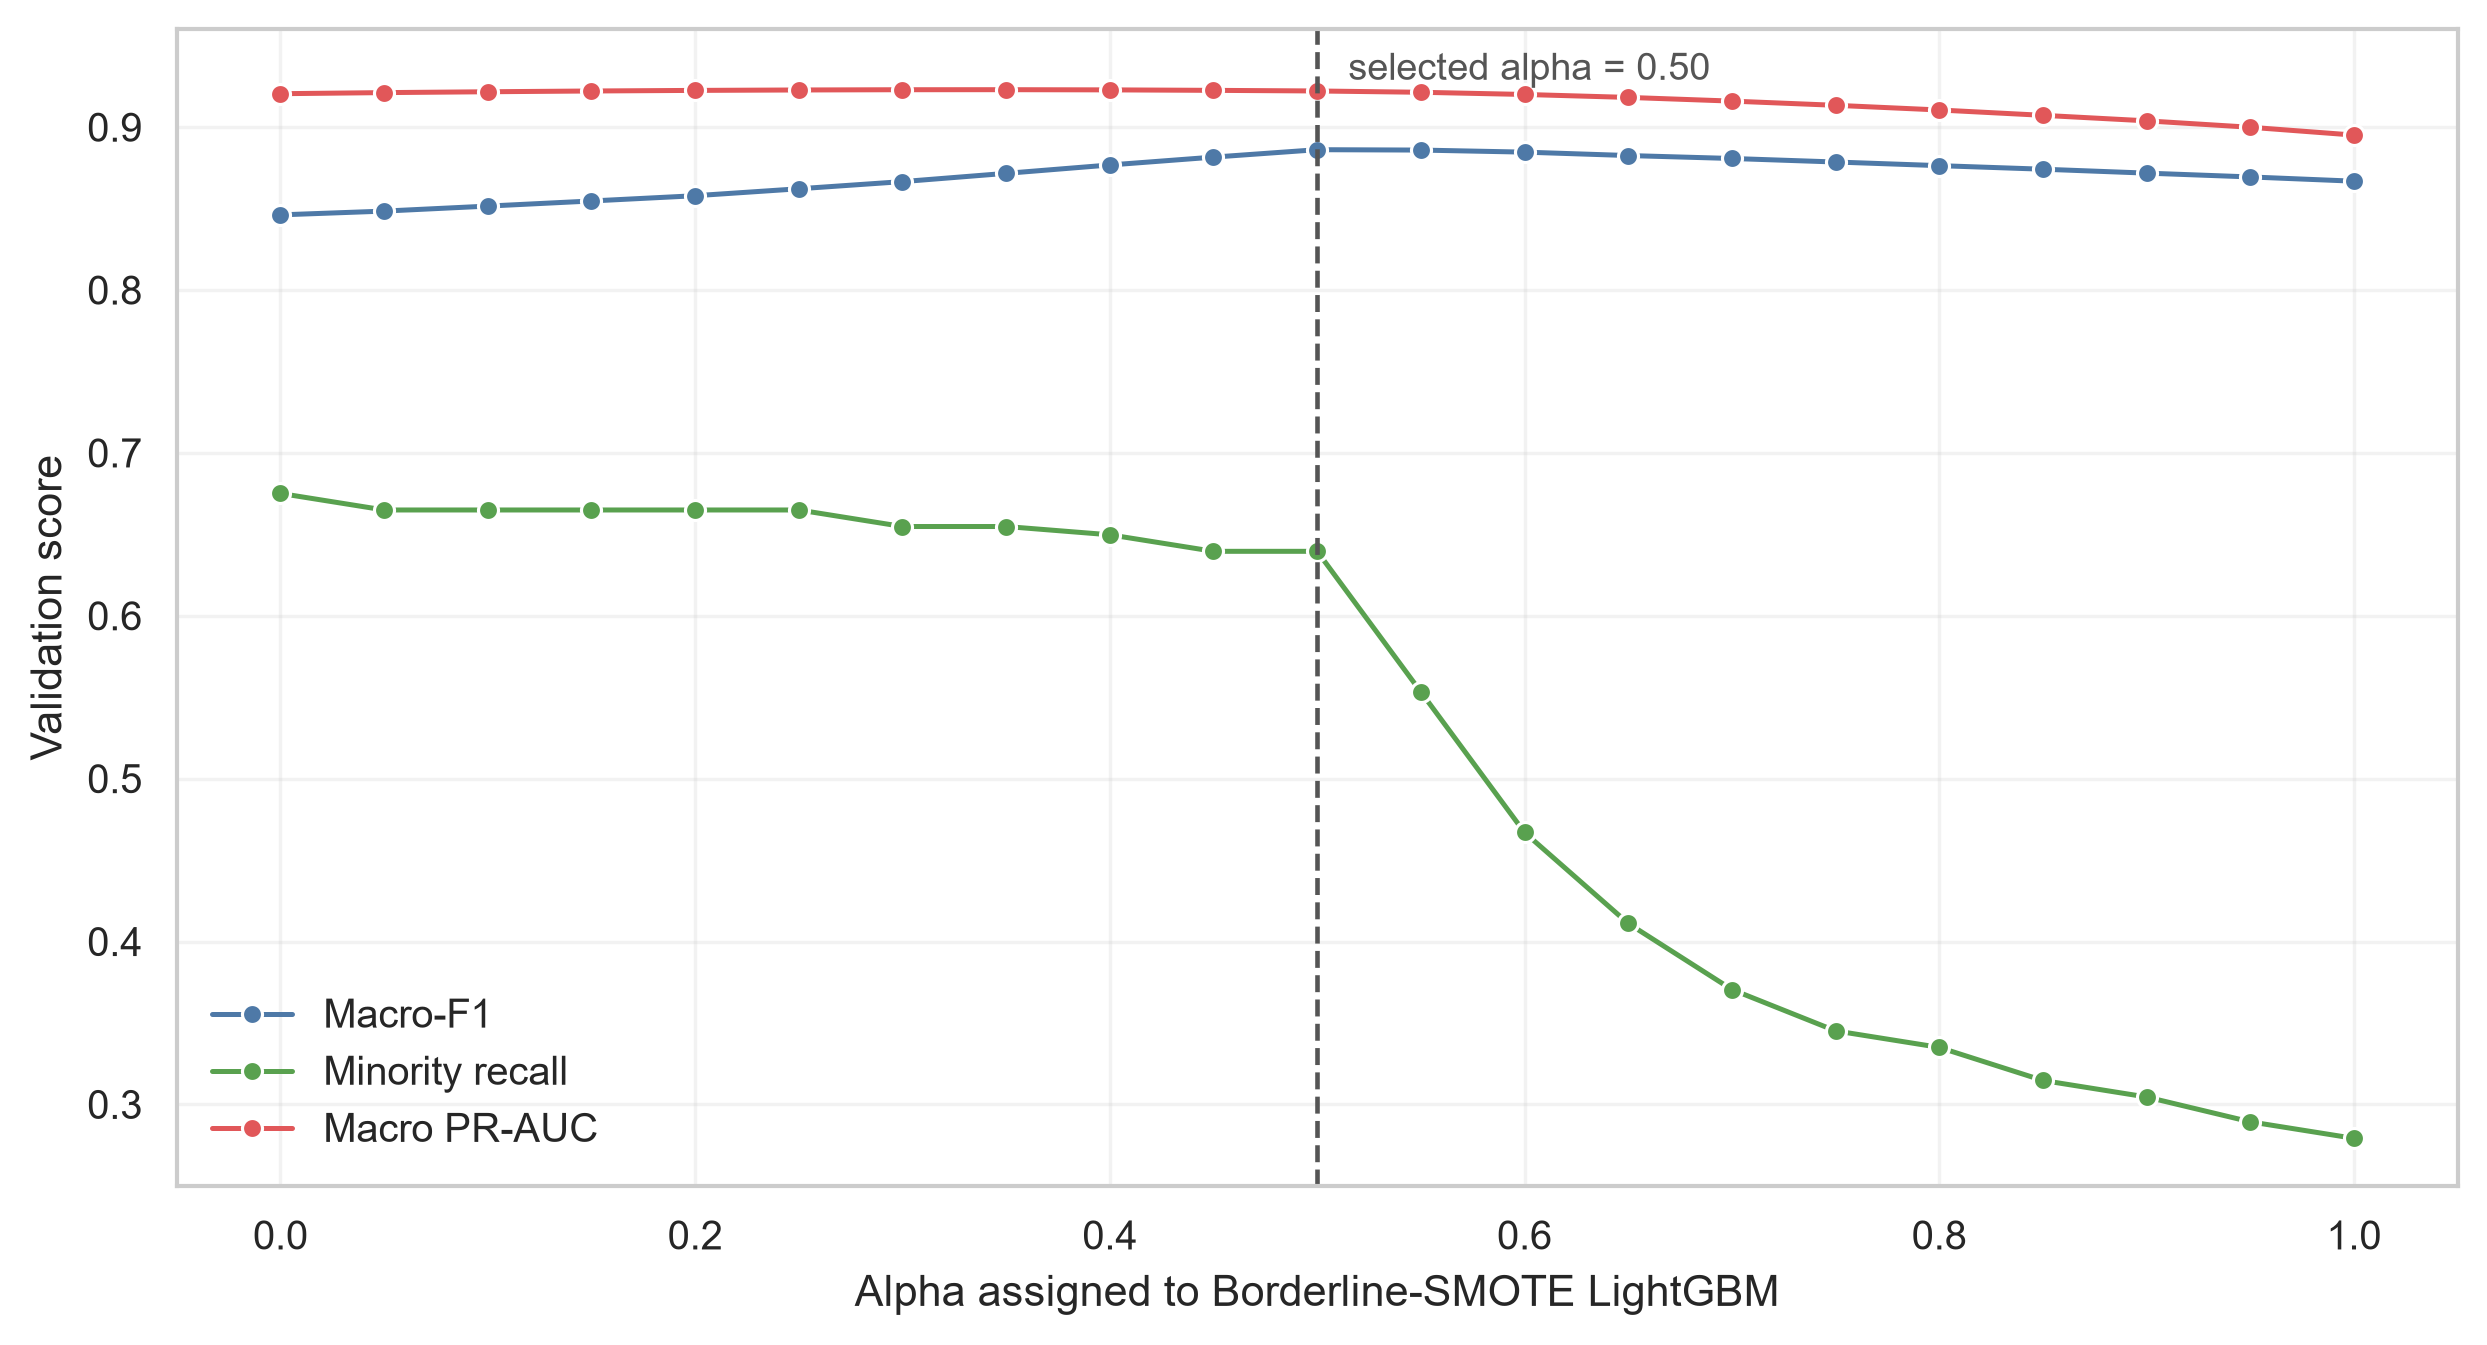
\includegraphics[width=0.82\linewidth]{figures/supplementary_figure_s2_ciciot_alpha_sensitivity.png}
\par\smallskip
\small Validation-subsplit Macro-F1, minority recall and macro PR-AUC across candidate ensemble weights. The selected value was $\alpha=0.50$ for the Borderline-SMOTE LightGBM component.
\end{center}

\section*{Supplementary Table S1. CICIoT2023 baseline variants}

\begin{center}
\scriptsize
\begin{tabular}{lccccc}
\toprule
Model & Accuracy & Balanced accuracy & Macro-F1 & Minority recall & Macro PR-AUC \\
\midrule
Flat LightGBM & 0.9462 & 0.8446 & 0.8612 & 0.1910 & 0.8863 \\
Random oversampling LightGBM & 0.9465 & 0.8439 & 0.8602 & 0.2247 & 0.8841 \\
Borderline-SMOTE LightGBM & 0.9477 & 0.8495 & 0.8674 & 0.2584 & 0.8933 \\
SMOTE LightGBM & 0.9469 & 0.8452 & 0.8622 & 0.2097 & 0.8902 \\
Weighted XGBoost & 0.9359 & 0.8981 & 0.8453 & 0.6592 & 0.9203 \\
Validation-controlled ensemble & 0.9486 & 0.8883 & 0.8828 & 0.5131 & 0.9219 \\
\bottomrule
\end{tabular}
\end{center}

\section*{Supplementary Table S2. IoTID20 split-bootstrap deltas}

\begin{center}
\tiny
\begin{longtable}{llccccc}
\toprule
Run ID & Metric & Mean delta & 2.5\% quantile & 97.5\% quantile & Splits & Resamples \\
\midrule
\endhead
iotid\_fine\_lgbm\_mi\_top10\_weighted & balanced\_accuracy & 0.0568 & 0.0546 & 0.0592 & 10 & 10000 \\
iotid\_fine\_lgbm\_xgb\_validation\_ensemble & balanced\_accuracy & 0.0566 & 0.0542 & 0.0591 & 10 & 10000 \\
iotid\_fine\_xgb\_weighted & balanced\_accuracy & 0.0548 & 0.0527 & 0.0572 & 10 & 10000 \\
iotid\_fine\_lgbm\_weighted & balanced\_accuracy & 0.0533 & 0.0511 & 0.0556 & 10 & 10000 \\
iotid\_fine\_lgbm\_mi\_top10\_flat & balanced\_accuracy & 0.0033 & 0.0021 & 0.0045 & 10 & 10000 \\
iotid\_fine\_lgbm\_mi\_top10\_weighted & f1\_macro & 0.0140 & 0.0117 & 0.0165 & 10 & 10000 \\
iotid\_fine\_lgbm\_xgb\_validation\_ensemble & f1\_macro & 0.0138 & 0.0114 & 0.0163 & 10 & 10000 \\
iotid\_fine\_lgbm\_weighted & f1\_macro & 0.0123 & 0.0102 & 0.0144 & 10 & 10000 \\
iotid\_fine\_xgb\_weighted & f1\_macro & 0.0116 & 0.0094 & 0.0139 & 10 & 10000 \\
iotid\_fine\_lgbm\_mi\_top10\_flat & f1\_macro & 0.0031 & 0.0020 & 0.0042 & 10 & 10000 \\
iotid\_fine\_lgbm\_weighted & minority\_recall\_mean & 0.2162 & 0.2117 & 0.2214 & 10 & 10000 \\
iotid\_fine\_xgb\_weighted & minority\_recall\_mean & 0.2132 & 0.2099 & 0.2163 & 10 & 10000 \\
iotid\_fine\_lgbm\_mi\_top10\_weighted & minority\_recall\_mean & 0.2129 & 0.2075 & 0.2178 & 10 & 10000 \\
iotid\_fine\_lgbm\_xgb\_validation\_ensemble & minority\_recall\_mean & 0.2128 & 0.2077 & 0.2173 & 10 & 10000 \\
iotid\_fine\_lgbm\_mi\_top10\_flat & minority\_recall\_mean & -0.0012 & -0.0017 & -0.0008 & 10 & 10000 \\
iotid\_fine\_lgbm\_mi\_top10\_flat & pr\_auc\_macro & 0.0019 & 0.0016 & 0.0022 & 10 & 10000 \\
iotid\_fine\_lgbm\_mi\_top10\_weighted & pr\_auc\_macro & 0.0001 & -0.0002 & 0.0004 & 10 & 10000 \\
iotid\_fine\_lgbm\_xgb\_validation\_ensemble & pr\_auc\_macro & 0.0001 & -0.0002 & 0.0004 & 10 & 10000 \\
iotid\_fine\_lgbm\_weighted & pr\_auc\_macro & -0.0016 & -0.0018 & -0.0014 & 10 & 10000 \\
iotid\_fine\_xgb\_weighted & pr\_auc\_macro & -0.0023 & -0.0027 & -0.0021 & 10 & 10000 \\
\bottomrule
\end{longtable}
\end{center}

\section*{Supplementary Table S3. IoTID20 exact sign-flip tests}

\begin{center}
\tiny
\begin{longtable}{llccccc}
\toprule
Run ID & Metric & Mean delta & Positive splits & Negative splits & Zero splits & Exact two-sided $p$ \\
\midrule
\endhead
iotid\_fine\_lgbm\_mi\_top10\_weighted & f1\_macro & 0.0140 & 10 & 0 & 0 & 0.0020 \\
iotid\_fine\_lgbm\_xgb\_validation\_ensemble & f1\_macro & 0.0138 & 10 & 0 & 0 & 0.0020 \\
iotid\_fine\_lgbm\_weighted & f1\_macro & 0.0123 & 10 & 0 & 0 & 0.0020 \\
iotid\_fine\_xgb\_weighted & f1\_macro & 0.0116 & 10 & 0 & 0 & 0.0020 \\
iotid\_fine\_lgbm\_mi\_top10\_flat & f1\_macro & 0.0031 & 9 & 1 & 0 & 0.0039 \\
iotid\_fine\_lgbm\_weighted & minority\_recall\_mean & 0.2162 & 10 & 0 & 0 & 0.0020 \\
iotid\_fine\_xgb\_weighted & minority\_recall\_mean & 0.2132 & 10 & 0 & 0 & 0.0020 \\
iotid\_fine\_lgbm\_mi\_top10\_weighted & minority\_recall\_mean & 0.2129 & 10 & 0 & 0 & 0.0020 \\
iotid\_fine\_lgbm\_xgb\_validation\_ensemble & minority\_recall\_mean & 0.2128 & 10 & 0 & 0 & 0.0020 \\
iotid\_fine\_lgbm\_mi\_top10\_flat & minority\_recall\_mean & -0.0012 & 0 & 9 & 1 & 0.0039 \\
iotid\_fine\_lgbm\_mi\_top10\_flat & pr\_auc\_macro & 0.0019 & 10 & 0 & 0 & 0.0020 \\
iotid\_fine\_lgbm\_mi\_top10\_weighted & pr\_auc\_macro & 0.0001 & 5 & 5 & 0 & 0.5156 \\
iotid\_fine\_lgbm\_xgb\_validation\_ensemble & pr\_auc\_macro & 0.0001 & 5 & 5 & 0 & 0.6523 \\
iotid\_fine\_lgbm\_weighted & pr\_auc\_macro & -0.0016 & 0 & 10 & 0 & 0.0020 \\
iotid\_fine\_xgb\_weighted & pr\_auc\_macro & -0.0023 & 0 & 10 & 0 & 0.0020 \\
\bottomrule
\end{longtable}
\end{center}

\section*{Supplementary Table S4. CICIoT2023 SHAP feature contributions}

\begin{center}
\small
\begin{tabular}{r l c c}
\toprule
Rank & Feature & Mean absolute SHAP & LightGBM gain \\
\midrule
1 & IAT & 0.5893 & 35188.0 \\
2 & Number & 0.5501 & 9861.0 \\
3 & Header\_Length & 0.2686 & 27253.0 \\
4 & Protocol Type & 0.1689 & 18648.0 \\
5 & rst\_count & 0.1605 & 18709.0 \\
6 & Weight & 0.1408 & 3422.0 \\
7 & syn\_count & 0.1354 & 18901.0 \\
8 & flow\_duration & 0.1243 & 29979.0 \\
9 & syn\_flag\_number & 0.1171 & 1138.0 \\
10 & Min & 0.1168 & 17946.0 \\
11 & Tot size & 0.1162 & 15534.0 \\
12 & Variance & 0.1106 & 9005.0 \\
13 & urg\_count & 0.0971 & 21191.0 \\
14 & Rate & 0.0859 & 31449.0 \\
15 & Magnitue & 0.0803 & 8659.0 \\
16 & fin\_count & 0.0780 & 7324.0 \\
17 & Max & 0.0662 & 11669.0 \\
18 & Tot sum & 0.0590 & 11090.0 \\
19 & Covariance & 0.0551 & 11545.0 \\
20 & Duration & 0.0480 & 24389.0 \\
\bottomrule
\end{tabular}
\end{center}

\section*{Supplementary Table S5. CICIoT2023 bootstrap summary}

\begin{center}
\scriptsize
\begin{longtable}{lcccc}
\toprule
Quantity & Point estimate & 2.5\% quantile & 97.5\% quantile & Resamples \\
\midrule
\endhead
baseline\_macro\_f1 & 0.8612 & 0.8580 & 0.8642 & 2000 \\
baseline\_balanced\_accuracy & 0.8446 & 0.8417 & 0.8477 & 2000 \\
baseline\_minority\_recall & 0.1910 & 0.1429 & 0.2385 & 2000 \\
baseline\_worst\_class\_recall & 0.1910 & 0.1429 & 0.2385 & 2000 \\
ensemble\_macro\_f1 & 0.8828 & 0.8801 & 0.8853 & 2000 \\
ensemble\_balanced\_accuracy & 0.8883 & 0.8854 & 0.8914 & 2000 \\
ensemble\_minority\_recall & 0.5131 & 0.4549 & 0.5714 & 2000 \\
ensemble\_worst\_class\_recall & 0.5131 & 0.4549 & 0.5651 & 2000 \\
delta\_macro\_f1 & 0.0216 & 0.0186 & 0.0246 & 2000 \\
delta\_balanced\_accuracy & 0.0437 & 0.0410 & 0.0465 & 2000 \\
delta\_minority\_recall & 0.3221 & 0.2635 & 0.3837 & 2000 \\
delta\_worst\_class\_recall & 0.3221 & 0.2635 & 0.3798 & 2000 \\
\bottomrule
\end{longtable}
\end{center}

The full bootstrap sample table is supplied as \path{supplementary_tables/ciciot_bootstrap_samples.csv}.

\section*{Supplementary Table S6. CICIoT2023 alpha grid}

\begin{center}
\scriptsize
\begin{longtable}{ccccc}
\toprule
Alpha & Macro-F1 & Minority recall & Macro PR-AUC & Composite score \\
\midrule
\endhead
0.00 & 0.8462 & 0.6751 & 0.9206 & 0.9002 \\
0.05 & 0.8485 & 0.6650 & 0.9212 & 0.9017 \\
0.10 & 0.8515 & 0.6650 & 0.9218 & 0.9047 \\
0.15 & 0.8547 & 0.6650 & 0.9222 & 0.9079 \\
0.20 & 0.8579 & 0.6650 & 0.9226 & 0.9111 \\
0.25 & 0.8622 & 0.6650 & 0.9228 & 0.9154 \\
0.30 & 0.8666 & 0.6548 & 0.9230 & 0.9190 \\
0.35 & 0.8717 & 0.6548 & 0.9230 & 0.9240 \\
0.40 & 0.8768 & 0.6497 & 0.9229 & 0.9288 \\
0.45 & 0.8816 & 0.6396 & 0.9226 & 0.9328 \\
0.50 & 0.8862 & 0.6396 & 0.9222 & 0.9373 \\
0.55 & 0.8859 & 0.5533 & 0.9214 & 0.9302 \\
0.60 & 0.8847 & 0.4670 & 0.9201 & 0.9220 \\
0.65 & 0.8826 & 0.4112 & 0.9183 & 0.9155 \\
0.70 & 0.8808 & 0.3706 & 0.9160 & 0.9104 \\
0.75 & 0.8786 & 0.3452 & 0.9134 & 0.9062 \\
0.80 & 0.8764 & 0.3350 & 0.9106 & 0.9032 \\
0.85 & 0.8742 & 0.3147 & 0.9073 & 0.8994 \\
0.90 & 0.8718 & 0.3046 & 0.9039 & 0.8962 \\
0.95 & 0.8695 & 0.2893 & 0.9000 & 0.8926 \\
1.00 & 0.8668 & 0.2792 & 0.8952 & 0.8892 \\
\bottomrule
\end{longtable}
\end{center}

\section*{Supplementary Table S7. Runtime and model complexity}

\begin{center}
\tiny
\setlength{\tabcolsep}{2pt}
\begin{longtable}{p{2.4cm}p{3.0cm}p{2.8cm}cccc}
\toprule
Dataset & Scope & Model & Train s & Inference ms per 10,000 & Model size KB & Peak memory MB \\
\midrule
\endhead
CICIoT2023 public subsample & full confirmatory split & Flat LightGBM & 136.1 & 1612.6 & 41698.0 & not measured \\
CICIoT2023 public subsample & full confirmatory split & Borderline-SMOTE LightGBM & 156.7 & 1715.0 & 41656.2 & not measured \\
CICIoT2023 public subsample & full confirmatory split & Weighted XGBoost & 278.0 & 275.6 & 24288.8 & not measured \\
CICIoT2023 public subsample & full confirmatory split & Validation controlled ensemble & 392.7 & 894.1 & 65945.0 & not measured \\
IoTID20 public mirror & mean across 10 repeated 70/30 splits & Top ten weighted LightGBM & 8.3 & 183.7 & not aggregated & not measured \\
IoTID20 public mirror & mean across 10 repeated 70/30 splits & Validation controlled ensemble & 26.4 & 125.5 & not aggregated & not measured \\
IoTID20 public mirror & mean across 10 repeated 70/30 splits & Weighted LightGBM & 12.2 & 189.9 & not aggregated & not measured \\
IoTID20 public mirror & mean across 10 repeated 70/30 splits & Weighted XGBoost & 18.6 & 65.8 & not aggregated & not measured \\
IoTID20 public mirror & mean across 10 repeated 70/30 splits & Top ten flat LightGBM & 8.1 & 183.3 & not aggregated & not measured \\
IoTID20 public mirror & mean across 10 repeated 70/30 splits & Flat LightGBM & 11.9 & 187.5 & not aggregated & not measured \\
CICIoT2023 public subsample & stratified quick screen, train\_n=220000, test\_n=80000 & Flat MLP & 5.8 & 9.3 & 131.2 & not measured \\
IoTID20 public mirror & stratified 70/30 quick screen & Flat MLP & 11.7 & 6.9 & 56.8 & not measured \\
\bottomrule
\end{longtable}
\end{center}

Peak memory was not measured in the current reproducibility run. This is retained as a transparent limitation rather than replaced with an estimate.

\section*{Supplementary Table S8. Hyperparameters and implementation details}

Core hyperparameters are supplied in \path{supplementary_tables/HYPERPARAMETER_TABLE.md}. The final CICIoT2023 public subsample ensemble used Borderline-SMOTE LightGBM and class weighted XGBoost probability outputs with validation selected alpha equal to 0.50. Borderline-SMOTE used adaptive \path{k_neighbors} from 1 to 5 according to the smallest class in the training split and the imbalanced learn default \path{m_neighbors}.

\section*{Supplementary Table S9. Short labels for Figure 2b}

\begin{center}
\small
\begin{tabular}{ll}
\toprule
Display label & Original CICIoT2023 public subsample label \\
\midrule
Uploading & Uploading\_Attack \\
Ping sweep & Recon-PingSweep \\
Backdoor & Backdoor\_Malware \\
XSS & XSS \\
\bottomrule
\end{tabular}
\end{center}

\section*{Supplementary Table S10. Device codes for Figure 4}

\begin{center}
\small
\begin{tabular}{ll}
\toprule
Device code & Original N-BaIoT held out device name \\
\midrule
D1 & Danmini\_Doorbell \\
D2 & Ecobee\_Thermostat \\
D3 & Ennio\_Doorbell \\
D4 & Philips\_B120N10\_Baby\_Monitor \\
D5 & Provision\_PT\_737E\_Security\_Camera \\
D6 & Provision\_PT\_838\_Security\_Camera \\
D7 & Samsung\_SNH\_1011\_N\_Webcam \\
D8 & SimpleHome\_XCS7\_1002\_WHT\_Security\_Camera \\
D9 & SimpleHome\_XCS7\_1003\_WHT\_Security\_Camera \\
\bottomrule
\end{tabular}
\end{center}

\section*{Supplementary Table S11. Benchmark context against recent intrusion detection studies}

\begin{center}
\tiny
\setlength{\tabcolsep}{2pt}
\begin{longtable}{p{1.4cm}p{2.0cm}p{2.0cm}p{1.9cm}p{2.5cm}p{1.6cm}p{2.1cm}p{2.6cm}}
\toprule
Study & Dataset or task & Model family & Imbalance handling & Validation and boundary test & Uncertainty & Main limitation for direct comparison & Present distinction \\
\midrule
\endhead
Alsubaei 2025 & NSL-KDD, UNSW-NB15, CICIDS2017 and related IDS benchmarks & XGBoost and optimized sequential neural network & Class imbalance considered through model and data choices & Cross validation and train test experiments; no split bootstrap or device held out test reported in the extracted manuscript & Not reported as paired uncertainty & Different datasets and task definitions; headline scores not directly comparable & Present study adds rare recall, frozen test selection, IoTID20 repeated holdouts and N-BaIoT device holdouts \\
Yu et al. 2025 & NSL-KDD and CIC-IDS2017 & Feature selection with CNN-LSTM & Equalized loss style class imbalance treatment & Repeated or fold based evaluation; no independent device holdout reported in the extracted manuscript & No paired split uncertainty table found & Strong architecture focus but less emphasis on frozen validation selection & Present study focuses on validation discipline and rare label diagnostics \\
Amine et al. 2025 & IoT intrusion detection benchmarks & Deep learning based IDS & Benchmark specific imbalance handling & Extensive benchmark figures and tables & No row bootstrap or split bootstrap reported in the extracted manuscript & Model novelty focus; validation boundary less explicit & Present study treats validation controls as the main contribution \\
Ma et al. 2025 & NF-ToN-IoT-v2, NF-UNSW-NB15-v2, NF-BoT-IoT-v2, NF-CSE-CIC-IDS2018-v2 and CIC-ToN-IoT & Feature selection, synthetic samples and LightGBM & Focal loss and synthetic minority support & Multiple datasets and train test validation & No paired uncertainty table found in the extracted manuscript & Strong multi dataset framing, but incompatible feature spaces and tasks & Present study complements this route with split and device boundary tests \\
Sarwar et al. 2025 & N-BaIoT and UNSW-NB15 & Decision tree, SVM, random forest and neural network & Feature selection and conventional classifiers & Five fold style evaluation and runtime reporting & No leave one device out N-BaIoT boundary reported in the extracted manuscript & Strong deployment context, but device transfer boundary is less direct & Present study uses complete held out devices in N-BaIoT \\
Singh et al. 2025 & Smart grid intrusion detection data & Attentional LSTM ensemble & Severe minority class treatment with large recall gains in its task & Domain specific training and evaluation & Uncertainty treatment differs from this study & Different domain and label granularity, so scores are not a direct CICIoT2023 comparison & Present study positions rare recall gains under public IoT benchmark validation \\
Abu-Shareha et al. 2026 & Supervised IDS literature & Review and multi criteria evaluation & Reviews imbalance as an evaluation dimension & Not an empirical detector & Not applicable & No new model result & Present study supplies an empirical validation controlled case \\
\bottomrule
\end{longtable}
\end{center}

This matrix is a benchmark context rather than a leaderboard. The studies differ in datasets, label granularity, task definitions and split protocols, so headline accuracy and detection rate are not directly comparable with the CICIoT2023 public subsample Macro-F1 reported in the main manuscript.

\section*{Supplementary Table S12. Model family and baseline screen}

\begin{center}
\tiny
\setlength{\tabcolsep}{2pt}
\begin{longtable}{p{2.1cm}p{3.0cm}p{2.4cm}cccccc}
\toprule
Dataset & Scope & Model & Features & Macro-F1 & Minority recall & Macro PR-AUC & Train s & Inference ms per 10,000 \\
\midrule
\endhead
CICIoT2023 public subsample & stratified quick three component ensemble screen, 220000 train and 80000 test rows & Three component ensemble screen & 46 & 0.8875 & 0.5733 & 0.9152 & 310.7 & 1559.2 \\
CICIoT2023 public subsample & stratified quick three component ensemble screen, 220000 train and 80000 test rows & Three component ensemble screen & 46 & 0.8875 & 0.5733 & 0.9152 & 310.7 & 1559.2 \\
CICIoT2023 public subsample & stratified quick three component ensemble screen, 220000 train and 80000 test rows & Three component ensemble screen & 46 & 0.8875 & 0.5733 & 0.9152 & 310.7 & 1559.2 \\
CICIoT2023 public subsample & stratified quick model family screen, 220000 train and 80000 test rows & Borderline-SMOTE LightGBM & 46 & 0.8797 & 0.4464 & 0.9058 & 31.0 & 1393.0 \\
CICIoT2023 public subsample & stratified quick model family screen, 220000 train and 80000 test rows & Weighted XGBoost & 46 & 0.8637 & 0.5536 & 0.9127 & 45.4 & 239.5 \\
CICIoT2023 public subsample & stratified quick model family screen, 220000 train and 80000 test rows & Hierarchical LightGBM & 20 & 0.8565 & 0.5536 & -- & 14.5 & 11758.0 \\
CICIoT2023 public subsample & stratified quick model family screen, 220000 train and 80000 test rows & Flat LightGBM & 46 & 0.8473 & 0.1250 & 0.8747 & 27.1 & 1345.0 \\
CICIoT2023 public subsample & stratified quick model family screen, 220000 train and 80000 test rows & Weighted Random Forest & 46 & 0.8421 & 0.5536 & 0.8702 & 8.1 & 166.1 \\
CICIoT2023 public subsample & stratified quick SMOTEENN screen, 220000 train and 80000 test rows & SMOTEENN LightGBM & 46 & 0.8082 & 0.7067 & 0.8495 & 86.8 & 1394.8 \\
CICIoT2023 public subsample & stratified quick model family screen, 220000 train and 80000 test rows & Weighted CatBoost & 46 & 0.7921 & 0.2857 & 0.8435 & 108.1 & 13.7 \\
CICIoT2023 public subsample & stratified quick model family screen, 220000 train and 80000 test rows & Weighted ExtraTrees & 46 & 0.7707 & 0.2321 & 0.8112 & 6.2 & 176.1 \\
CICIoT2023 public subsample & stratified quick screen, train\_n=220000, test\_n=80000 & Flat MLP & 46 & 0.5361 & 0.0000 & 0.5744 & 5.8 & 9.3 \\
IoTID20 public mirror & stratified 70/30 quick model family screen & Top ten weighted LightGBM & 10 & 0.6209 & 0.4908 & 0.6784 & 9.9 & 204.0 \\
IoTID20 public mirror & stratified 70/30 quick model family screen & Weighted LightGBM & 22 & 0.6186 & 0.4986 & 0.6768 & 14.1 & 209.2 \\
IoTID20 public mirror & stratified 70/30 quick model family screen & Weighted XGBoost & 22 & 0.6177 & 0.4803 & 0.6764 & 21.5 & 73.5 \\
IoTID20 public mirror & stratified 70/30 quick model family screen & Weighted CatBoost & 22 & 0.6163 & 0.4504 & 0.6786 & 56.9 & 6.4 \\
IoTID20 public mirror & stratified 70/30 quick model family screen & Flat LightGBM & 22 & 0.6103 & 0.2637 & 0.6784 & 14.0 & 215.3 \\
IoTID20 public mirror & stratified 70/30 quick model family screen & Weighted Random Forest & 22 & 0.6054 & 0.4689 & 0.6562 & 15.0 & 69.7 \\
IoTID20 public mirror & stratified 70/30 quick screen & Flat MLP & 22 & 0.4937 & 0.0380 & 0.5750 & 11.7 & 6.9 \\
\bottomrule
\end{longtable}
\end{center}

The model family screen includes quick CICIoT2023 public subsample and IoTID20 checks, additional tree baselines and a simple MLP baseline. It is not used to replace the full frozen CICIoT2023 public subsample result in the main manuscript.

\section*{Supplementary Table S13. CICIoT2023 public subsample hardest and easiest class diagnostics}

\begin{center}
\tiny
\setlength{\tabcolsep}{2pt}
\begin{longtable}{p{2.7cm}p{2.5cm}cccccc}
\toprule
Diagnostic group & Class & Support & Flat recall & Ensemble recall & Recall delta & Flat F1 & Ensemble F1 \\
\midrule
\endhead
hardest by ensemble recall & Uploading\_Attack & 267 & 0.1910 & 0.5131 & 0.3221 & 0.2506 & 0.4521 \\
hardest by ensemble recall & XSS & 729 & 0.3827 & 0.5761 & 0.1934 & 0.4282 & 0.5357 \\
hardest by ensemble recall & Backdoor\_Malware & 640 & 0.4719 & 0.6406 & 0.1688 & 0.5167 & 0.6129 \\
hardest by ensemble recall & CommandInjection & 1086 & 0.4401 & 0.6621 & 0.2219 & 0.5010 & 0.6815 \\
hardest by ensemble recall & Recon-PingSweep & 465 & 0.4065 & 0.6667 & 0.2602 & 0.5136 & 0.6072 \\
hardest by ensemble recall & Recon-OSScan & 9953 & 0.6749 & 0.6995 & 0.0246 & 0.7435 & 0.7592 \\
hardest by ensemble recall & SqlInjection & 1028 & 0.5409 & 0.7208 & 0.1800 & 0.6077 & 0.6767 \\
hardest by ensemble recall & BrowserHijacking & 1155 & 0.6667 & 0.7273 & 0.0606 & 0.7523 & 0.7116 \\
hardest by ensemble recall & DictionaryBruteForce & 2543 & 0.7157 & 0.7703 & 0.0547 & 0.7555 & 0.7283 \\
hardest by ensemble recall & Recon-PortScan & 9934 & 0.7725 & 0.7746 & 0.0021 & 0.7656 & 0.7772 \\
hardest by ensemble recall & DNS\_Spoofing & 9990 & 0.7605 & 0.7855 & 0.0250 & 0.7882 & 0.8003 \\
hardest by ensemble recall & MITM-ArpSpoofing & 10072 & 0.8402 & 0.8417 & 0.0016 & 0.8819 & 0.8823 \\
easiest non benign by ensemble recall & DDoS-RSTFINFlood & 10162 & 1.0000 & 1.0000 & 0.0000 & 1.0000 & 1.0000 \\
easiest non benign by ensemble recall & Mirai-udpplain & 10074 & 0.9997 & 0.9999 & 0.0002 & 0.9999 & 0.9999 \\
easiest non benign by ensemble recall & DDoS-PSHACK\_Flood & 10042 & 0.9999 & 0.9999 & 0.0000 & 1.0000 & 1.0000 \\
easiest non benign by ensemble recall & DDoS-ICMP\_Flood & 9925 & 0.9999 & 0.9999 & 0.0000 & 0.9999 & 0.9999 \\
easiest non benign by ensemble recall & DDoS-SynonymousIP\_Flood & 9845 & 0.9999 & 0.9999 & 0.0000 & 0.9995 & 0.9995 \\
easiest non benign by ensemble recall & DDoS-ACK\_Fragmentation & 9998 & 0.9998 & 0.9998 & 0.0000 & 0.9998 & 0.9998 \\
easiest non benign by ensemble recall & DoS-TCP\_Flood & 10067 & 0.9997 & 0.9997 & 0.0000 & 0.9997 & 0.9997 \\
easiest non benign by ensemble recall & DDoS-ICMP\_Fragmentation & 10088 & 0.9995 & 0.9996 & 0.0001 & 0.9998 & 0.9998 \\
easiest non benign by ensemble recall & DDoS-UDP\_Flood & 10050 & 0.9996 & 0.9996 & 0.0000 & 0.9995 & 0.9996 \\
easiest non benign by ensemble recall & DDoS-TCP\_Flood & 9967 & 0.9997 & 0.9996 & -0.0001 & 0.9997 & 0.9997 \\
easiest non benign by ensemble recall & Mirai-greip\_flood & 10076 & 0.9995 & 0.9995 & 0.0000 & 0.9990 & 0.9993 \\
easiest non benign by ensemble recall & DoS-UDP\_Flood & 9982 & 0.9993 & 0.9995 & 0.0002 & 0.9995 & 0.9996 \\
\bottomrule
\end{longtable}
\end{center}

\section*{Supplementary Table S14. CICIoT2023 public subsample low support class diagnostics}

\begin{center}
\tiny
\setlength{\tabcolsep}{2pt}
\begin{longtable}{p{3.0cm}ccccccc}
\toprule
Class & Support & Flat precision & Flat recall & Flat F1 & Ensemble precision & Ensemble recall & Ensemble F1 \\
\midrule
\endhead
Uploading\_Attack & 267 & 0.3643 & 0.1910 & 0.2506 & 0.4041 & 0.5131 & 0.4521 \\
Recon-PingSweep & 465 & 0.6974 & 0.4065 & 0.5136 & 0.5576 & 0.6667 & 0.6072 \\
Backdoor\_Malware & 640 & 0.5709 & 0.4719 & 0.5167 & 0.5874 & 0.6406 & 0.6129 \\
XSS & 729 & 0.4861 & 0.3827 & 0.4282 & 0.5006 & 0.5761 & 0.5357 \\
SqlInjection & 1028 & 0.6933 & 0.5409 & 0.6077 & 0.6377 & 0.7208 & 0.6767 \\
CommandInjection & 1086 & 0.5815 & 0.4401 & 0.5010 & 0.7021 & 0.6621 & 0.6815 \\
BrowserHijacking & 1155 & 0.8632 & 0.6667 & 0.7523 & 0.6965 & 0.7273 & 0.7116 \\
DictionaryBruteForce & 2543 & 0.8000 & 0.7157 & 0.7555 & 0.6905 & 0.7703 & 0.7283 \\
DDoS-SlowLoris & 4642 & 0.9966 & 0.9974 & 0.9970 & 0.9970 & 0.9991 & 0.9981 \\
DDoS-HTTP\_Flood & 5766 & 0.9988 & 0.9964 & 0.9976 & 0.9986 & 0.9967 & 0.9977 \\
VulnerabilityScan & 7546 & 0.9984 & 0.9991 & 0.9987 & 0.9985 & 0.9991 & 0.9988 \\
DDoS-SynonymousIP\_Flood & 9845 & 0.9991 & 0.9999 & 0.9995 & 0.9992 & 0.9999 & 0.9995 \\
\bottomrule
\end{longtable}
\end{center}

\section*{Supplementary Table S15. IoTID20 repeated split class wise diagnostics}

\begin{center}
\tiny
\setlength{\tabcolsep}{2pt}
\begin{longtable}{p{2.4cm}p{2.6cm}cccccc}
\toprule
Class & Model & Mean support & Mean recall & SD recall & Mean F1 & Recall delta & F1 delta \\
\midrule
\endhead
DoS-Synflooding & Flat LightGBM & 17817.0 & 0.9992 & 0.0002 & 0.9995 & -0.0001 & -0.0001 \\
DoS-Synflooding & Top ten flat LightGBM & 17817.0 & 0.9992 & 0.0002 & 0.9995 & -0.0001 & -0.0001 \\
DoS-Synflooding & Top ten weighted LightGBM & 17817.0 & 0.9992 & 0.0002 & 0.9995 & -0.0001 & -0.0001 \\
DoS-Synflooding & Validation controlled ensemble & 17817.0 & 0.9992 & 0.0002 & 0.9995 & -0.0001 & -0.0001 \\
DoS-Synflooding & Weighted XGBoost & 17817.0 & 0.9992 & 0.0002 & 0.9995 & -0.0001 & -0.0001 \\
MITM ARP Spoofing & Flat LightGBM & 10613.0 & 0.4659 & 0.0042 & 0.5535 & 0.2042 & 0.0045 \\
MITM ARP Spoofing & Top ten flat LightGBM & 10613.0 & 0.4612 & 0.0032 & 0.5504 & 0.2042 & 0.0045 \\
MITM ARP Spoofing & Top ten weighted LightGBM & 10613.0 & 0.6701 & 0.0047 & 0.5580 & 0.2042 & 0.0045 \\
MITM ARP Spoofing & Validation controlled ensemble & 10613.0 & 0.6706 & 0.0043 & 0.5578 & 0.2042 & 0.0045 \\
MITM ARP Spoofing & Weighted XGBoost & 10613.0 & 0.6731 & 0.0045 & 0.5446 & 0.2042 & 0.0045 \\
Mirai-Ackflooding & Flat LightGBM & 16537.0 & 0.2161 & 0.0386 & 0.2251 & 0.3510 & 0.1543 \\
Mirai-Ackflooding & Top ten flat LightGBM & 16537.0 & 0.2333 & 0.0353 & 0.2437 & 0.3510 & 0.1543 \\
Mirai-Ackflooding & Top ten weighted LightGBM & 16537.0 & 0.5671 & 0.0470 & 0.3794 & 0.3510 & 0.1543 \\
Mirai-Ackflooding & Validation controlled ensemble & 16537.0 & 0.5672 & 0.0480 & 0.3791 & 0.3510 & 0.1543 \\
Mirai-Ackflooding & Weighted XGBoost & 16537.0 & 0.5340 & 0.0313 & 0.3720 & 0.3510 & 0.1543 \\
Mirai-HTTP Flooding & Flat LightGBM & 16746.0 & 0.2463 & 0.0431 & 0.2497 & 0.0203 & 0.0152 \\
Mirai-HTTP Flooding & Top ten flat LightGBM & 16746.0 & 0.2544 & 0.0478 & 0.2609 & 0.0203 & 0.0152 \\
Mirai-HTTP Flooding & Top ten weighted LightGBM & 16746.0 & 0.2666 & 0.0453 & 0.2648 & 0.0203 & 0.0152 \\
Mirai-HTTP Flooding & Validation controlled ensemble & 16746.0 & 0.2644 & 0.0449 & 0.2631 & 0.0203 & 0.0152 \\
Mirai-HTTP Flooding & Weighted XGBoost & 16746.0 & 0.2977 & 0.0270 & 0.2829 & 0.0203 & 0.0152 \\
Mirai-Hostbruteforceg & Flat LightGBM & 36354.0 & 0.7673 & 0.0047 & 0.7084 & -0.2632 & -0.0559 \\
Mirai-Hostbruteforceg & Top ten flat LightGBM & 36354.0 & 0.7618 & 0.0052 & 0.7049 & -0.2632 & -0.0559 \\
Mirai-Hostbruteforceg & Top ten weighted LightGBM & 36354.0 & 0.5041 & 0.0037 & 0.6526 & -0.2632 & -0.0559 \\
Mirai-Hostbruteforceg & Validation controlled ensemble & 36354.0 & 0.5038 & 0.0039 & 0.6524 & -0.2632 & -0.0559 \\
Mirai-Hostbruteforceg & Weighted XGBoost & 36354.0 & 0.4861 & 0.0029 & 0.6379 & -0.2632 & -0.0559 \\
Mirai-UDP Flooding & Flat LightGBM & 55066.0 & 0.7681 & 0.0134 & 0.7761 & -0.0644 & 0.0500 \\
Mirai-UDP Flooding & Top ten flat LightGBM & 55066.0 & 0.7760 & 0.0157 & 0.7816 & -0.0644 & 0.0500 \\
Mirai-UDP Flooding & Top ten weighted LightGBM & 55066.0 & 0.7037 & 0.0012 & 0.8261 & -0.0644 & 0.0500 \\
Mirai-UDP Flooding & Validation controlled ensemble & 55066.0 & 0.7037 & 0.0012 & 0.8261 & -0.0644 & 0.0500 \\
Mirai-UDP Flooding & Weighted XGBoost & 55066.0 & 0.7037 & 0.0012 & 0.8261 & -0.0644 & 0.0500 \\
Normal & Flat LightGBM & 12022.0 & 0.9697 & 0.0010 & 0.9840 & 0.0008 & -0.0007 \\
Normal & Top ten flat LightGBM & 12022.0 & 0.9698 & 0.0009 & 0.9839 & 0.0008 & -0.0007 \\
Normal & Top ten weighted LightGBM & 12022.0 & 0.9705 & 0.0009 & 0.9833 & 0.0008 & -0.0007 \\
Normal & Validation controlled ensemble & 12022.0 & 0.9705 & 0.0009 & 0.9833 & 0.0008 & -0.0007 \\
Normal & Weighted XGBoost & 12022.0 & 0.9687 & 0.0008 & 0.9823 & 0.0008 & -0.0007 \\
Scan Hostport & Flat LightGBM & 6658.0 & 0.2691 & 0.0030 & 0.4011 & 0.2129 & -0.0416 \\
Scan Hostport & Top ten flat LightGBM & 6658.0 & 0.2679 & 0.0030 & 0.3998 & 0.2129 & -0.0416 \\
Scan Hostport & Top ten weighted LightGBM & 6658.0 & 0.4820 & 0.0081 & 0.3595 & 0.2129 & -0.0416 \\
Scan Hostport & Validation controlled ensemble & 6658.0 & 0.4819 & 0.0078 & 0.3596 & 0.2129 & -0.0416 \\
Scan Hostport & Weighted XGBoost & 6658.0 & 0.4824 & 0.0065 & 0.3583 & 0.2129 & -0.0416 \\
Scan Port OS & Flat LightGBM & 15922.0 & 0.6736 & 0.0139 & 0.5760 & 0.0492 & 0.0007 \\
Scan Port OS & Top ten flat LightGBM & 15922.0 & 0.6808 & 0.0098 & 0.5768 & 0.0492 & 0.0007 \\
Scan Port OS & Top ten weighted LightGBM & 15922.0 & 0.7228 & 0.0066 & 0.5766 & 0.0492 & 0.0007 \\
Scan Port OS & Validation controlled ensemble & 15922.0 & 0.7231 & 0.0062 & 0.5767 & 0.0492 & 0.0007 \\
Scan Port OS & Weighted XGBoost & 15922.0 & 0.7236 & 0.0065 & 0.5744 & 0.0492 & 0.0007 \\
\bottomrule
\end{longtable}
\end{center}

\section*{Supplementary Table S16. N-BaIoT cap sensitivity}

\begin{center}
\tiny
\setlength{\tabcolsep}{2pt}
\begin{longtable}{ccccccccc}
\toprule
Cap & Task & Run ID & Folds & Mean F1 & Min F1 & Mean present F1 & Min present recall & Mean PR-AUC \\
\midrule
\endhead
5000 & attack & nb\_attack\_lgbm\_importance\_top40\_weighted & 9 & 0.9193 & 0.8137 & 0.9348 & 0.0014 & 0.9655 \\
5000 & attack & nb\_attack\_lgbm\_mi\_top40\_weighted & 9 & 0.9325 & 0.8143 & 0.9325 & 0.0014 & 0.9642 \\
5000 & attack & nb\_attack\_lgbm\_weighted & 9 & 0.9388 & 0.8526 & 0.9388 & 0.0014 & 0.9652 \\
20000 & attack & nb\_attack\_lgbm\_weighted & 9 & 0.9435 & 0.7483 & 0.9867 & 0.6917 & 0.9902 \\
50000 & attack & nb\_attack\_lgbm\_weighted & 9 & 0.9948 & 0.9855 & 0.9948 & 0.8767 & 0.9960 \\
5000 & binary & nb\_binary\_lgbm\_weighted & 9 & 0.9832 & 0.8613 & 0.9832 & 0.9355 & -- \\
20000 & binary & nb\_binary\_lgbm\_weighted & 9 & 0.9998 & 0.9993 & 0.9998 & 0.9990 & -- \\
5000 & family & nb\_family\_lgbm\_weighted & 9 & 0.9998 & 0.9992 & 0.9998 & 0.9984 & 1.0000 \\
20000 & family & nb\_family\_lgbm\_weighted & 9 & 0.9999 & 0.9995 & 0.9999 & 0.9990 & 1.0000 \\
\bottomrule
\end{longtable}
\end{center}

The 50,000 row per file sensitivity was run for the fine grained attack task because binary and family settings were already near saturated at the smaller caps.

\section*{Supplementary Table S17. CICIoT2023 rare prior operating point screen}

\begin{center}
\tiny
\setlength{\tabcolsep}{2pt}
\begin{longtable}{ccccccccc}
\toprule
Objective & Alpha & Rare scope & Multiplier & Accuracy & Macro-F1 & Minority recall & Macro PR-AUC & Worst class \\
\midrule
\endhead
macro\_f1 & 0.50 & lowest\_support & 1.00 & 0.9450 & 0.8875 & 0.5733 & 0.9152 & Recon-PingSweep \\
macro\_f1\_plus\_minority & 0.50 & lowest\_support & 4.00 & 0.9447 & 0.8803 & 0.6000 & 0.9149 & XSS \\
recall\_sensitive & 0.50 & lowest\_support & 6.00 & 0.9446 & 0.8787 & 0.6400 & 0.9147 & XSS \\
minority\_recall\_constrained & 0.50 & lowest\_support & 6.00 & 0.9446 & 0.8787 & 0.6400 & 0.9147 & XSS \\
\bottomrule
\end{longtable}
\end{center}

The source for this table is the quick stratified screen. Rare prior tuning multiplies probabilities for the lowest support label or labels selected from the training split and selects the multiplier on an internal validation split. It is reported as a recall sensitive operating point, not as a replacement for the primary Macro-F1 operating point.

\section*{Reproduction commands}

\begin{verbatim}
.\.venv\Scripts\python.exe scripts\run_ciciot_confirmatory_experiments.py `
  --out-dir ciciot_confirmatory_full
.\.venv\Scripts\python.exe scripts\run_ciciot_recall_aware_ensemble.py `
  --out-dir ciciot_ensemble_full
.\.venv\Scripts\python.exe scripts\run_ciciot_rare_prior_tuning.py `
  --out-dir ciciot_rare_prior_tuning_full
.\.venv\Scripts\python.exe scripts\run_ciciot_smoteenn_ensemble.py `
  --train-n 220000 --test-n 80000 --out-dir ciciot_ensemble_smoteenn_quick
.\.venv\Scripts\python.exe scripts\run_iotid20_repeated_split_uncertainty.py
.\.venv\Scripts\python.exe scripts\run_nbaiot_unseen_device.py `
  --n-per-file 20000 --out-dir nbaiot_unseen_device_20k `
  --run-id nb_binary_lgbm_weighted `
  --run-id nb_family_lgbm_weighted `
  --run-id nb_attack_lgbm_weighted
.\.venv\Scripts\python.exe scripts\run_ciciot_explainability.py `
  --shap-sample 3000
.\.venv\Scripts\python.exe scripts\run_ciciot_bootstrap_uncertainty.py `
  --n-bootstrap 2000 --out-dir statistical_uncertainty
.\.venv\Scripts\python.exe scripts\run_mlp_baselines.py `
  --out-dir mlp_baselines
.\.venv\Scripts\python.exe scripts\make_result_figures.py
\end{verbatim}

\end{document}
